\section{Mathematical Foundation}

Note: The order \(n\) of a point \(P\) is a number such that \(nP = \infty\) and creates
the cyclic subgroup \(\langle P \rangle = \{ \infty, P, 2P, ..., (n-1)P \} \).

Note: Add something about wNAF multiplication? \verb+http://link.springer.com/chapter/10.1007%2F978-3-540-68914-0_26#page-1+

\subsection{Curves and Point Arithmetic}
\label{sec:math_curve}

\subsubsection{Weierstrass Curves}

Weierstrass simple form is very easy to perform operations on. This is also the one
BouncyCastle primarily supports (\verb|FpCurve|). Weierstrass curves are of the form
\(y^2 = x^3 + ax + b\). Arithmetic operations on points in a curve of the Weierstrass
simple form are fairly easy to implement.
\paragraph{Addition}

Addition of two points \(P + Q = R\) is a fairly straight-forward matter. Given two points, \(P = (x_1,y_1)\) and
\(Q = (x_2,y_2)\), the result \(R = (x_3,y_3)\) can be found with the following calculations:

\begin{equation}
	\lambda = {{y_2-y_1} \over {x_2-x_1}}
\end{equation}

\begin{equation}
	x_3 = \lambda^2 - x_1 - x_2 \textbf{ and } y_3 = \lambda (x_1 - x_3) - y_1
\end{equation}

As elliptic curves also contain the \(\infty\) (infinity) point, there is a single exception to this
rule: if either \(P\) or \(Q\) is infinity, the result of adding them will be infinity, too.

\begin{equation}
    Q = \infty \lor P = \infty \implies P + Q = \infty\
\end{equation}

\paragraph{Doubling}

If the points being added are equal to one another (\(P + Q = R \text{, where } P = Q \text{ and } P = (x_1,y_1)\)),
the result can be calculated with a simplified formula:

\begin{equation}
	\lambda = {{3x_1^2 + a} \over {2y_1}} \text{, where } a \text { is the parameter from the curve formula }
\end{equation}

\begin{equation}
	x_3 = \lambda^2 - 2x_1 \textbf{ and } y_3 = \lambda (x_1 - x_3) - y_1
\end{equation}

The resulting point is then \(R = (x_3, y_3)\).

\paragraph{Subtraction}

A subtraction \(P - Q = R\) can be expressed through addition and negation, as \(P - Q = P + (-Q)\). Negation of a given point
\(P = (x,y)\) is calculated as \(-P = (x,-y)\) (a reflection over the x-axis).

As with addition, negation is complicated by the existence of the infinity point:

\begin{equation}
	-\infty = \infty \textbf{ and } P - P = \infty
\end{equation}

The negation of infinity is infinity (negative infinity does not exist), and a point subtracted from itself is infinity.\cite{hankerson2010}

\subsubsection{Scalar Multiplication}

Scalar multiplication of a point \(P\) and an integer \(d\) is, with the most simple algorithm, calculated through repeated addition
of the point to an accumulator. Several algorithms to speed up this process exist, and as point multiplication is most computational
time is spent\footnote{See Section \ref{sec:performance_components} for a confirmation of this.} a few are covered in the following:
\emph{Double-and-Add}, \emph{NAF}, and \emph{wNAF}.

\paragraph{Double-and-Add}

The DoubleAndAdd method limits the number of additions necessary by doubling the accumulating result whenever possible, resulting in
fewer total additions.

The algorithm relies on first representing the number \(d\) in its binary form, \(d_{binary} = (d_{t-1}, ... , d_2, d_1, d_0)_2\),
where \(t\) is the number of bits used to represent the number. Each bit is then inspected, from least significant (right) to most
significant (left): if the bit is \(1\), the current value of \(P\) is added to the accumulator. For each bit inspected, \(P\) is
doubled.\cite{hankerson2010}

This algorithm results in \(~1.5t\) additions (most of which are doublings), much less than the \(~0.5t^2\) additions required for
repeatedly adding the point to an accumulator.

\paragraph{Non-adjacent form}

Whereas the binary form of a number is constructed from \(\{0,1\}\), the non-adjacent form (NAF) is constructed from \(\{-1,0,1\}\), with
the added limitation that no non-zero values are adjacent (hence the name). Subtraction of points is (almost) as efficient as addition,
requiring only an additional negation of a finite field element (see above).

The NAF of a number \(d\) can be constructed by an algorithm, which finds each digit as \(d_i = 2 - (d \text{ mod } 4)\) if \(d\) is odd, and
\(0\) otherwise. \(d\) is then reduced by \(d_i\) and halved, before the algorithm repeats for the next value. This continues until \(d < 1\).

The multiplication \(dP\) can be calculated using the \(NAF(d)\) with an appropriate algorithm (see Figure \ref{fig:naf-algorithm}).\cite{hankerson2010}

\begin{figure}[htb!]
	\centering
	\begin{tabular}{|p{\textwidth}|}
		\hline
		Input: Positive integer \(k\), \(P \in E(\mathbb{F}_q)\). \\
		Output: \(kP\).

		\begin{enumerate*}
			\item Compute \(NAF(k) = \Sigma^{l-1}_{i=0} k_i2^i\).
			\item \(Q \gets \infty\).
			\item For \(i\) from \(l-1\) downto \(0\) do
			\begin{enumerate*}
				\item \(Q \gets 2Q\).
				\item If \(k_i = 1\) then \(Q \gets Q + P\).
				\item If \(k_1 = -1\) then \(Q \gets Q - P\).
			\end{enumerate*}
			\item Return(\(Q\)).
		\end{enumerate*}
		\\
		\hline
	\end{tabular}
	\caption{The algorithm for computing the scalar multiplication \(kP\) using the non-adjacent form of \(k\), as represented by
		Hankerson et.al.\cite{hankerson2010}}
	\label{fig:naf-algorithm}
\end{figure}

The running time for the NAF algorithm is approximately \(1 {1 \over 3} l\), where \(l\) is the length of the NAF, quicker than that
of the Double-and-Add.\cite{hankerson2010}

\paragraph{Windowed NAF}

The NAF can be improved further by allowing a wider range of values than just those in \(\{-1,0,1\}\). The range is called a \emph{window}, and
using this windowed non-adjacent form (wNAF) can improve running time, but requires some pre-computation. Regular \(NAF\) is the same
as \(wNAF_2\) (a window size of 2), and \(wNAF_3\) would be constructed from the values \(\{-3,-1,0,1,3\}\).

The wNAF of an integer is calculated in much the same way as a NAF, but with some added complexity due to the variable size of \(w\)
(see Figure \ref{fig:compute-wnaf-algorithm}).

\begin{figure}[htb!]
	\begin{tabular}{|p{\textwidth}|}
		\hline
		Input: Window width \(w\), positive integer \(k\). \\
		Output: \(NAF_w(k)\).
		\begin{enumerate*}
			\item \(i \gets 0\).
			\item While \(k \geq 1\) do
			\begin{enumerate*}
				\item If \(k\) is odd then: \(k_i \gets k \text{ mods } 2^w\), \(k \gets k - k_i\);
				\item Else: \(k_i \gets 0\).
				\item \(k \gets k/2\), \(i \gets i + 1\).
			\end{enumerate*}
			\item Return(\(k_{i-1},k_{i-2},...,k_1,k_0\)).
		\end{enumerate*} \\
		\hline
		Where \(k \text{ mods } 2^w\) is: 
		\begin{enumerate*}
			\item If \(k \text{ mod } 2^w \geq 2^{w-1}\) then return(\((k \text{ mod } 2^w) - 2^w\));
			\item Else return(\(k \text{ mod } 2^w\)).
		\end{enumerate*} \\
		\hline
	\end{tabular}
	\caption{The algorithm for constructing a wNAF representation of an integer \(k\), as represented by Hankerson
		et.al.\cite{hankerson2010} Here with added explanation of \(k \text{ mods } 2^w\).}
	\label{fig:compute-wnaf-algorithm}
\end{figure}

The wNAF multiplication algorithm relies on the precomputation of the values \(P_i = iP \text{ for } i \in \{1,3,5,...,2^{w-1}-1\}\). If the
point \(P\) is fixed for many operations, then this precomputation may be worthwhile, even at big values for \(w\). For dynamically varying
\(P\) (such as in asymmetric encryption) a large \(w\) may result in an overhead larger than the benefit of the quicker operations.

The wNAF multiplication algorithm is very similar to that of the regular NAF, distinguishing itself by its precomputation and slightly more
advanced structure for non-zero \(k_i\) (see Figure \ref{fig:wnaf-algorithm}).

\begin{figure}[htb!]
	\begin{tabular}{|p{\textwidth}|}
		\hline
		Input: Window width \(w\), positive integer \(k\), \(P \in E(\mathbb{F}_q)\).\\
		Output: \(kP\).
		\begin{enumerate*}
			\item Compute \(wNAF_w(k) = \Sigma^{l-1}_{i=0} k_i 2^i\).
			\item Compute \(P_i = iP\) for \(i \in \{1,3,5,...,2^{w-1}-1\}\).
			\item \(Q \gets \infty\).
			\item For \(i\) from \(l - 1\) downto \(0\) do
			\begin{enumerate*}
				\item \(Q \gets 2Q\).
				\item If \(k_i \neq 0\) then:
				\begin{enumerate*}
					\item If \(k_i > 0\) then \(Q \gets Q + P_{k_i}\);
					\item Else \(Q \gets Q - P_{-k_i}\).
				\end{enumerate*}
			\end{enumerate*}
			\item Return(\(Q\)).
		\end{enumerate*} \\
		\hline
	\end{tabular}
	\caption{Algorithm for computing the multiplication \(kP\) using the wNAF algorithm, as represented by Hankerson et.al.\cite{hankerson2010}}
	\label{fig:wnaf-algorithm}
\end{figure}

wNAF is a generalization of NAF, and so the formula for running time of wNAF is a generalization of the running time for NAF. The number of
additions performed in wNAF depends on the window \(w\) and can be described as \(2^{w-2} + (1 + {1 \over {w + 1}}) l\), where \(l\) is the length
of the wNAF form.

\subsection{Encoding}
\label{sec:math_encoding}

Some elliptic curve based cryptosystems (such as the adapted ElGamal in Section \ref{sec:math_encryption}) are constructed to encrypt points on a curve. To make
this useful an original string message must be encoded as a point. The encoding must be reversible.

It is trivial to map a message string to the correct numberspace as both strings and numbers have binary representations. The number is then
simply found by converting a string to its binary representation and interpreting this as an integer. Using the ASCII character set the string
\verb+"A"+ is mapped to the number \verb+65+.

\begin{verbatim}
    string_to_binary "A" -> 1000001
    binary_to_integer 1000001 ->  65
\end{verbatim}

Koblitz is attributed with an algorithm that maps a message \(m\), represented as an integer in \(\mathbb{Z}_p\), to a point on the curve of the
simple Weierstrass form \(y^2 = x^3 + ax + b \text{ mod } p\).\cite{MappingAMessage}

An integer K is selected such that \((M + 1)K < p\), and this is used to compute
a candidate x-coordinate for the point, \(x_j = MK + j \text{ mod } p\). To verify the validity of the candidate, a check is performed: \(x_j\)
is a valid x-coordinate for a point on the curve if \(z_j = x_j^3 + ax_j + b\) has a square root. If the candidate is valid, the message \(m\)
can be mapped to a point \(M\) on the curve:

\begin{equation}
	M = (x_j, y_j) \text{, where } y_j = \sqrt{z_j} \text{ mod } p
\end{equation}

If no square root exists for \(z_j\) for all \(j\), \(j = 0 \text{ to } K-1\), then it is not possible to map the message to a point. In other
words, the method is probablistic and it is possible that a message cannot be encoded.

To find the original message from a point again, a simple calculcation is performed:

\begin{equation}
	m = {\lfloor {x \over K} \rfloor}
\end{equation}

The flooring of \(x \over K\) ensures that any \(j\) added to \(MK\) has no effect.\cite{MappingAMessage}

As the numberspace the messages must be mapped to is limited by the size of the prime field \(\mathbb{F}_p\) over which the curve is defined, so is the
length of the message. The numeric value of a string can be no greater than \(p\).

\paragraph{Picking the value K}

The selection of value \(K\) has implications on both the probability that a message can be mapped, and the performance of the encoding algoirthm.
The probability of successful encoding is described as \(P_{success} \geq 1 - {1 \over {2^K}}\): the larger the value of \(K\), the greater the probability,
as shown in Figure \ref{fig:probability}. With \(K\) greater than 6, no discernible change in probability occurs.\cite{MappingAMessage}

\begin{figure}[htb]
	\centering
	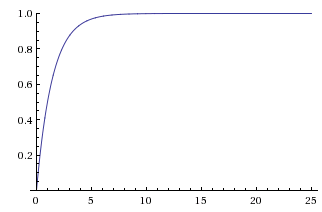
\includegraphics[width=0.6\textwidth]{maths/encoding-probability}
	\caption{Minimum probability of successful encoding, depending on size of K. (Illustrated with http://www.wolframalpha.com)}
	\label{fig:probability}
\end{figure}

The performance of the mapping depends on three calculations: (1) the multiplication \(MK\); (2) the calculation of \(z_j\), specifically
performing the calculations \(x_j^3\) and \(ax_j\); and (3) the computation of a potential root \(\sqrt{z_j}\). While the first calculation (1)
is performed only once, the last two (2,3) are repeated until a root is found, or all possible values have been tried.

Multiplication is a heavy operation, and picking a smaller value of \(K\) limits both the load of each multiplications (as they are performed with
smaller numbers), and the number of multiplications (as the range of \(j\)s used is limited by \(K - 1\)). So while it is easy to find the greatest
possible value \(K_greatest = {\lfloor { p \over {MK} }\rfloor}\), yielding the highest probability of success, this is not necessarily desirable.
Picking \(K = 7\) gives a probability of success \(P_{success} \geq 0.993\) -- high enough for our purposes.
\subsection{Encryption}
\label{sec:math_encryption}

Public key encryption is often used to distribute keys for symmetric encryption schemes, as asymmetric encryption
is generally slower than symmetric encryption. Symmetric encryption cannot be used for the first contact between
two parties, and as such public key encryption is the first step of communicating secret data.

\subsubsection{ElGamal}

ElGamal is -- history -- public key cryptography -- stuff.

Traditional ElGamal uses pub and priv keys for... (maths!)

This can be adapted to elliptic curves, easily, by using ---

Differences are...

Required maths---